%%%%%%%%%%%%%%%%%%%%%%%%%%%%%%%%%%%%%%%%%%%%%%%%%%%%%%%%%%%%%%%%%%%%%%%
% Sample template for MIT Junior Lab Student Written Summaries
% Available from http://web.mit.edu/8.13/samplepaper/sample-paper.tex
%
% Last Updated June 20, 2004
%
% Adapted from the American Physical Societies REVTeK-4 Pages
% at http://publish.aps.org
%
% ADVICE TO STUDENTS: Each time you write a paper, start with this
%    template and save under a new filename.  If convenient, don't
%    erase unneeded lines, just comment them out.  Often, they
%    will be useful containers for information.
%%%%%%%%%%%%%%%%%%%%%%%%%%%%%%%%%%%%%%%%%%%%%%%%%%%%%%%%%%%%%%%%%%%%%%%


%%%%%%%%%%%%%%%%%%%%%%%%%%%%%%%%%%%%%%%%%%%%%%%%%%%%%%%%%%%%%%%%%%%%%%%
% PREAMBLE
% The preamble of a LaTeX document is the set of commands that precede
% the \begin{document} line.  It contains a \documentclass line
% to load the REVTeK-4 macro definitions and various \usepackage
% lines to load other macro packages.
%
% ADVICE TO STUDENTS: This preamble contains a suggested set of
%     class options to generate a ``Junior Lab'' look and feel that
%     facilitate quick review and feedback from one's peers, TA's
%     and section instructors.  Don't make substantial changes without
%     first consulting your section instructor.
%%%%%%%%%%%%%%%%%%%%%%%%%%%%%%%%%%%%%%%%%%%%%%%%%%%%%%%%%%%%%%%%%%%%%%%

\documentclass[aps,twocolumn,secnumarabic,nobalancelastpage,amsmath,amssymb,
nofootinbib]{revtex4}

% nofootinbib is another document class option that allows you to put
% footnotes on the page where they occur rather than at the end of the
% paper.  This makes for easier reading!

% secnumarabic is a particularly nice way of identifying sections by
% number to aid electronic review and commentary.

% amsmath and amssymb are necessary for the subequations environment
% among others

\usepackage{graphics}      % standard graphics specifications
\usepackage{graphicx}      % alternative graphics specifications
\usepackage{longtable}     % helps with long table options
\usepackage{url}           % for on-line citations
\usepackage{bm}            % special 'bold-math' package
\usepackage{subfigure}
\usepackage{booktabs}

%%%%%%%%%%%%%%%%%%%%%%%%%%%%%%%%%%%%%%%
%                                 %%%%%
% And now, begin the document...  %%%%%
%                                 %%%%%
%%%%%%%%%%%%%%%%%%%%%%%%%%%%%%%%%%%%%%%
\begin{document}
\title{Atomic Physics}
\author         {Kevin L. Chen. Partner: Tanooj Shah}
\affiliation    {UC Berkeley, Department of Physics}
\date{\today}

\begin{abstract}
Much of the Atomic, Molecular, and Optical (AMO) physics incorporate the fundamental concepts of energy levels and transitions. In this experiment, we explored two important effects arising from the structure of the atom: electron transitions and energy level degeneracy. We then looked for two constants that are important for each effect: the Rydberg Constant and the Bohr Magneton. For the first effect, electron transitions, we used a monochromator and diffraction grating to measure the wavelengths of Balmer Transitions for the Hydrogen atom. Through these calculations, we found the Rydberg Constant to be $1.094 \times 10^{7} \pm 2.28 \times 10^{5} $ m$^{-1}$. Then for the second part involving energy level degeneracies, we applied a magnetic field to a Helium discharge tube to see the Zeeman effect. By splitting the lines a certain amount and noting the magnetic field, we were able to determine the Bohr Magneton to be $8.752 \times 10^{-21} \pm 2.512 \times 10^{-21}$ ergs/G. We also explore possible errors in our experiment such as scratched lenses and spectral broadening.
\end{abstract}

\maketitle

%%%%%%%%%%%%%%%%%%%%%%%%%%%%%%%%%%%%%%%%%%%%%%%%%%%%%%%%%%%%%%%%%%%%%%%%%%%%%
\section*{Introduction}

Atomic Spectroscopy is one of the fundamental fields of physics where Quantum Mechanics its energy level became more robust theoretically. From atomic spectroscopy, physicists have discovered the Rydberg Formula, illustrating the transitions between electron energy levels. One of the most important of these transitions are called the Balmer Series, which depicts the transitions from n $>$ 3 states to n = 2 stages. The light from this series is visible light. Furthermore, by introducing a magnetic field to the atom, we add a new term to the Hamiltonian. This new term gives rise to Zeeman splitting. With this magnetic field, we see spectral lines splitting, due to a split in the energy levels. Using modern day optics and spectroscopic techniques, we can use these spectral lines to determine the Rydberg Constant and the Bohr Magneton. 
%%%%%%%%%%%%%%%%%%%%%%%%%%%%%%%%%%%%%%%%%%%%%%%%%%%%%%%%%%%%%%%%%%%%%%%%%%%%%
\section{Balmer Series}
\subsection{Theory}

To begin speaking about the Balmer Series, one must understand the Bohr Model. In this mode of an atom, the electron revolves around the nucleus of the atom, much like a planet revolves around the sun. Therefore, we have a force balance equation 

\begin{equation}
    {m_\mathrm{e} v^2\over r} = {Zk_\mathrm{e} e^2 \over r^2} 
   \label{Bohr Model}
\end{equation}

where $m_e$ is the electron's mass, $e$ is the charge of the electron, $k_e$ is Coulomb's constant and $Z$ is the atom's atomic number. However, unlike in classical mechanics where the angular momentum is continuous, quantum mechanics exhibits discrete values of angular momentum. Specifically, the angular momentum is an integer multiple of Planck's Constant:

\begin{equation}
     m_\mathrm{e} v r = n \hbar 
   \label{Quantized L}
\end{equation}

where $n$ is the Principle Quantum Number, denoting the state that the electron is in. 

By combining Equation~\ref{Bohr Model} and Equation~\ref{Quantized L}, we arrive at the relationship between the Principle Quantum number and the corresponding energy:

\begin{equation}
      E = - { Z^2(k_\mathrm{e} e^2)^2 m_\mathrm{e} \over 2\hbar^2 n^2} \approx {-13.6Z^2 \over n^2}\mathrm{eV}
   \label{Energy Level for nth Level}
\end{equation} 

The Balmer Series are the series of transitions where atoms end up in the $n = 2$ state. This means any transition from $n > 2$ to $n = 2$ is a Balmer Series transition. These transitions result in energy loss in the form of a photon, which is what we observed as visible spectrum lines. The energies of these photons are described by this energy difference relation, called the Rydberg Formula:

\begin{equation} 
    E=E_i-E_f=R_\mathrm{E} \left( \frac{1}{n_{f}^2} - \frac{1}{n_{i}^2} \right) \,
  \label{Rydberg Forumla}
\end{equation}

and since $ E = hc / \lambda $, the above equation can be rewritten as 

\begin{equation} 
    \frac{1}{\lambda}=R \left( \frac{1}{n_{f}^2} - \frac{1}{n_{i}^2} \right). \,
  \label{Use this Rydberg Formula}
\end{equation}

where $n_{f} = 2$ for the Balmer Series.

In this experiment, we use Equation~\ref{Use this Rydberg Formula} to determine the Rydberg Constant, $R$, by plotting $1 / \lambda$ against $1 / n^{2} $.

\subsection{Setup}

\begin{figure}[ht]
  \begin{center}
    \subfigure[Balmer Series Setup]{\label{Balmer}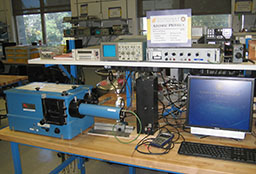
\includegraphics[width=6 cm]{BalmerSetup.jpg}}
    \subfigure[Grating in the Monochromator]{\label{Grating}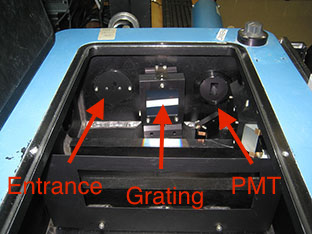
\includegraphics[width=6 cm]{Grating.jpg}} \\
  \end{center}
  \caption{Atomic Physics Experiment Setup at UC Berkeley}[\footnotesize{``Atomic Physics.'' - Physics 111-Lab Wiki. UC Berkeley, n.d. Web. 4 May. 2015.}]
  \label{ThreeFigs}
\end{figure}

For this part of the experiment, we used the following pieces of equipment:
\begin{itemize}
\item Hydrogen gas discharge tube
\item Mercury gas discharge tube
\item Monochromater with a 300 groove/mm reflective grating
\item Photomultiplier tube
\item Lens to focus the light
\item Oscilloscope and Multimeter
\item LabVIEW
\end{itemize}

To retrieve the spectrum, we used a lens with a focal length of 12 cm and concentrated the light into the entrance of the monochromator (Left side of Figure~\ref{Grating}). The light is reflected off of one mirror, onto the diffraction grating, and then onto another mirror out into the photomultiplier tube (mirrors not shown). The grating is a 300 groove per millimeter diffraction-grating, and the grooves are able to split the light into spectral lines with well-defined wavelengths (Figure~\ref{Reflective}). With this grating, we could observe different spectral lines of the Mercury and Hydrogen as they entered the monochromator automatically. 

\subsection{Procedure}
In the first part of the experiment, we measured the wavelengths of Balmer Series lines of Hydrogen. However, since we do not know the wavelengths of the Balmer Series of Hydrogen, we first found the spectral lines of Mercury to then superimpose the Hydrogen lines on top. The spectral lines of Mercury are known, so we can use those lines to calibrate the monochromator and find the Hydrogen spectral lines.

\begin{figure}[t]
  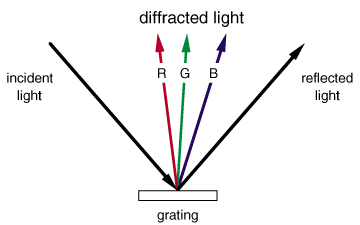
\includegraphics[width = 5 cm]{Diffraction.png}
  \begin{center}
  \caption{A reflective Diffraction Grating}[\footnotesize{``Diffraction Gratings – The Crucial Dispersive Component." Diffraction Gratings – The Crucial Dispersive Component. N.p., n.d. Web. 05 May 2015.}]
  \label{Reflective}
  \end{center}
\end{figure}

The monochromator we used comes equipped with the ability to automatically sweep through a range of wavelengths at a speed of $\Delta wavelength / \Delta t$. The feed from the PMT is then fed into LabVIEW, where we set the same sweep speed and are able to get the full visible spectrum of the Mercury gas from 300 nm to 700 nm light. We then repeated this process to find the spectral lines for Hydrogen. 

\subsection{Analysis}

\begin{figure*}[t]
  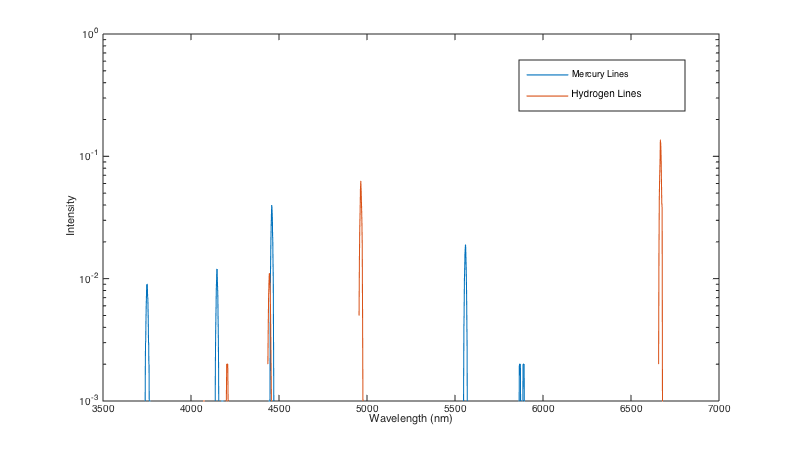
\includegraphics[width=\textwidth, height = 10 cm]{Balmer.png}
  \caption{Spectral Lines of Mercury and Hydrogen}
  \label{Spectrums}
\end{figure*}

After taking data of the spectral lines of both Mercury and Hydrogen, we superimposed the spectra on top of each other. The result is shown in Figure~\ref{Spectrums}. 

\begin{table}[h]
\begin{tabular}{|l|l|l|}
\hline
Recorded Wavelength & Actual  & Difference \\ \hline
4146                & 4046.56 & -99.44     \\
4458                & 4358.33 & -99.67     \\
5556                & 5460.74 & -95.26     \\
5868                & 5769.6  & -98.4      \\
5892                & 5790.66 & -101.34    \\
6252                & 6149.5  & -102.5     \\ \hline
\end{tabular}
\caption{Recorded Values of Mercury's Recorded Spectral Line Wavelengths and the difference between the value recorded by the monochromator and actual value.}
\label{Mercury Recorded vs Actual}
\end{table}

The data on the actual wavelengths of the peaks are recorded in Table~\ref{Mercury Recorded vs Actual}. In this table, we used the means of the peaks. When we looked at the difference between the actual wavelength against our recorded wavelength, we found that, on average, there was a -99.435 nm difference between the actual and recorded values for the Mercury spectrum. This -99.435 nm difference is what we used to estimate the actual values of the Hydrogen Balmer Series lines. 

\begin{table}[h]
\begin{tabular}{|l|l|l|}
\hline
Initial Energy State & Recorded Wavelength ($\AA$) & $\sigma$ ($\AA$)\\ \hline
3 & 6567                & 4.62               \\
4 & 4866                & 4.72               \\
5 & 4347                & 4.93               \\
6 & 4107                & 3.87               \\
7 & 3976                & 5.88               \\ \hline
\end{tabular}
\caption{Recorded Values of Hydrogen's Recorded Spectral Line Wavelengths and Standard Deviations of those Wavelengths. The photons with these wavelengths come from energy transitions indicated in the first column to energy level n = 2.}
\label{Hydrogen Recorded}
\end{table}

\begin{figure}[t]
  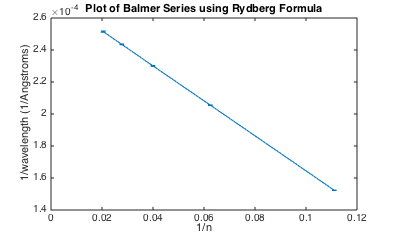
\includegraphics[width = 8 cm]{Rydberg.png}
  \begin{center}
  \caption{A plot of the Rydberg Formula with the data from Table~\ref{Hydrogen Recorded} with error bars}
  \label{Rydberg Plot}
  \end{center}
\end{figure}

When we repeated the procedure for the Hydrogen discharge tube, we recorded the values in Table~\ref{Hydrogen Recorded}. With this table and Equation~\ref{Use this Rydberg Formula}, we calculated the Rydberg Formula, which came out to be $1.094 \times 10^{7}$ m$^{-1}$ with a standard deviation of $2.28 \times 10^{5} $ m$^{-1}$.  

\subsection{Uncertainty}

Areas of uncertainty were in the due to the equipment and natural causes in broadening. We were unable to quantify how much the lens was able to distort our data. Some examples of uncertainties in our data can be found in the Appendix.

\subsubsection{Equipment}

The lens that we used to direct the light into the monochromater had scratches on it, which would cause the lens to act somewhat like a diffraction grating. This would cause some uncertainties in the spectral lines. 

\subsubsection{Broadening}

\begin{figure}[t]
  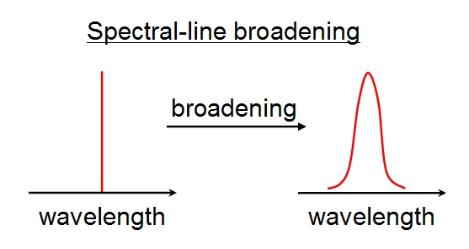
\includegraphics[width = 5 cm]{Broadening.jpg}
  \begin{center}
  \caption{Broadening, caused by several factors like natural broadening, thermal broadening, and collision broadening.}[\footnotesize{``CV Accretion Discs." CV Accretion Discs. N.p., n.d. Web. 24 Apr. 2015.}]
  \label{Broadening}
  \end{center}
\end{figure}

The effect that would be in every experiment, regardless of quality of optical equipment, would be spectral broadening. If each electron transition was just to emit a photon with a well defined energy and, thus, one wavelength, then the spectral line we ought to observe would be infinitely thin (Left side of Fig~\ref{Broadening}). However, several factors give the line a width: the uncertainty principle,

\begin{equation}
   \Delta{E}\Delta{t} \geq \frac{\hbar}{2} \Rightarrow \Delta \nu = \frac{1}{2 \pi \Delta t}
  \label{Natural Equation}
\end{equation}

thermal broadening,

\begin{equation}
  \Delta \nu = \sqrt{\frac{8kT\ln 2}{mc^2}}\nu_{0}
  \label{Doppler Equation}
\end{equation}

and collision broadening

\begin{equation}
  \Delta \nu = \sqrt{\frac{8kT}{m}} n \sigma
  \label{Collision Equation}
\end{equation}  

Natural broadening is caused by the Heisenberg Uncertainty Principle. Second, thermal Broadening is caused by the movement of the atoms. Since the gases that are being excited are moving, some atoms will be moving towards the observer, and thus emitting blue shifted light, while some atoms will move away from the observer will emit red shifted light. This frequency shifting is caused by thermal effects, and therefore is called Thermal Broadening. Last, spectral line broadening is also caused by collision broadening. If atoms that are emitting light are constantly colliding with other atoms, then their electron energy levels get spread out.

In Table~\ref{Spread}, we see that thermal broadening has the largest effect on the spread of the spectral line by almost three orders of magnitude. Since the values we used to calculate the spreads in the table are similar to the actual values in the experiment, we can assume that the largest cause in spread and uncertainty will be through thermal broadening. 

\begin{table}[h]
  \begin{tabular}{|l|l|}
  \hline
  Type of Broadening & FWHM Wavelength Spread          \\ \hline
  Natural            & 0.0150 picometers               \\
  Thermal            & 9.37 picometers                 \\
  Collision          & 0.0244 picometers               \\ \hline
  \end{tabular}
  \caption{The approximate spreads due to different types of broadening. Calculations were done with the frequency of red light ($400$ THz), P $= 5$ Torr, T $= 600$ K, and $\Delta t = 10$ ns}
  \label{Spread}
\end{table}

\section{Zeeman Effect}

\subsection{Theory}

Another quantum effect we observe in this experiment is the Zeeman Effect, where a weak magnetic field is applied to atoms, adding a term to their Hamiltonian, and thus splitting energy levels. 

We begin with the Hamiltonian of an atom: 

\begin{equation}
    H = H_0 -\vec{\mu} \cdot \vec{B}, \: \: \vec\mu =\frac{e}{2m_e}g\vec j
  \label{Hamiltonian}
\end{equation}

where $H_0$ is the unperturbed Hamiltonian and the second term is the term resulting from the Zeeman Effect. The other terms $\vec\mu$ are as follows: 

\begin{itemize}
 \item $e$ is the fundamental charge value
 \item $m_e$ is the mass of the electron
 \item $\vec B$ is the magnetic field
 \item $\vec j$ is the total angular momentum resulting from a sum of the electron's orbital angular momentum $\vec l$ and its spin angular momentum $\vec s$
 \item $g$ is the Lande-g Factor (a multiplicative factor that arises when a weak magnetic field is introduced to the atom.) given by:

\begin{equation}
  g_J \approx \frac{3}{2}+\frac{S(S+1)-L(L+1)}{2J(J+1)}. 
  \label{Lande G}
\end{equation}

\end{itemize}

By taking the dot product, we get the projection of the angular momentum $\vec j$ against the axis of the magnetic field, which results in the following energy perturbation:

\begin{equation} 
  \Delta E = \mu_0 B \Delta (g m_j)
  \label{Zeeman Energies}
\end{equation}

This $m_j$ terms are what the energy levels split into, and can take on the integral values from $-j$ to $+j$ depending on the j value. 

\begin{figure}[t]
  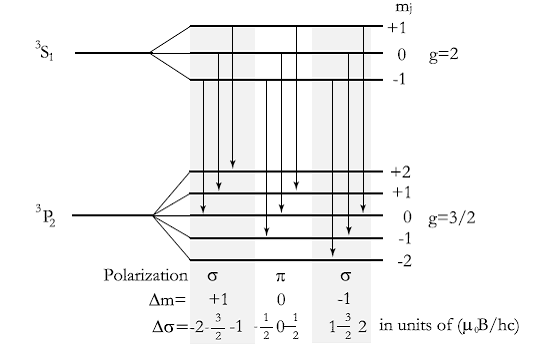
\includegraphics[width = 0.4\textwidth]{ZeemanSplitting.png}
  \begin{center}
  \caption{Structure of the Zeeman multiplet arising in a transition from a $^{3}S_1$ to a $^{3}P_2$ level.}[\footnotesize{``Atomic Physics.'' - Physics 111-Lab Wiki. UC Berkeley, n.d. Web. 23 Apr. 2015.}]
  \label{ZeemanSplitting}
  \end{center}
\end{figure}

An important part of this experiment is the Fabry -- P\'{e}rot interferometer, which is discussed in depth in Section~\ref{FPI}. A relation that arises from this device is the Free Spectral Range, which relates the wave number to the properties of the F--P interferometer. 

\begin{equation} 
  \Delta \sigma = \frac{\alpha}{2tn}
  \label{FP Equation}
\end{equation}

where $\alpha$ is a constant depending on how much Zeeman Splitting we induce, $n$ is the index of refraction of air, $t$ is the thickness of the interferometer, and $\sigma$ is the wave number. We also know through the deBroglie relations that 

\begin{equation}
  E = hc/\lambda 
  \label{deBroglie}
\end{equation}

and since $\lambda = 1 / \sigma$, then $E = hc\sigma$ and $\Delta E = hc \Delta \sigma$. A change in energy from Equation~\ref{Zeeman Energies} results in $\Delta E = \mu_0 B \Delta (m_j g)$. Relating this to Equation~\ref{FP Equation} and Equation~\ref{Zeeman Energies}, we get the relationship to find the Bohr Magneton:

\begin{equation}
  \mu_0 = \frac{h c \alpha}{2 t n B \Delta(g m_j)}
  \label{Bohr Magneton}
\end{equation}

\subsection{Setup}

\begin{figure}[h]
  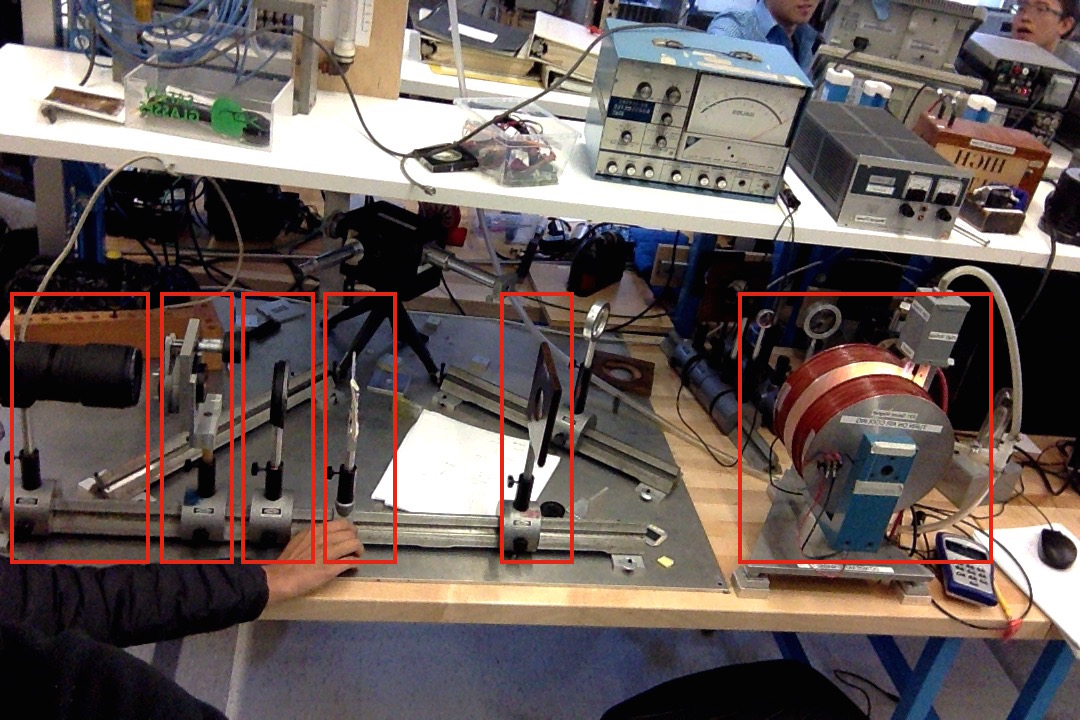
\includegraphics[width = 0.48\textwidth]{ZeemanSetup1.jpg}
  \begin{center}
  \caption{Setup for observing $\sigma$ and $\pi$ splitting. The red boxes indicate different pieces of equipment. From left to right: Camera, Fabry -- P\'{e}rot interferometer, rotating polarizer, red filter, focusing lens, Helmholtz coils, and between the coils is the Helium discharge tube. The light enters the interferometer and then exists, interfering with itself and creating Airy Disks.}
  \label{FP1}
  \end{center}
\end{figure}

For this part of the experiment, we used the following pieces of equipment:
\begin{itemize}
\item Helium gas discharge tube
\item 20K Gauss Helmholtz Coil
\item Red Filter
\item Fabry -- P\'{e}rot interferometer
\item Rotating Polarizer
\item Lens to focus the light
\item Camera
\item Prism Spectrometer
\item LabVIEW
\end{itemize}

\subsubsection{Fabry -- P\'{e}rot interferometer} \label{FPI}

\begin{figure}[t]
  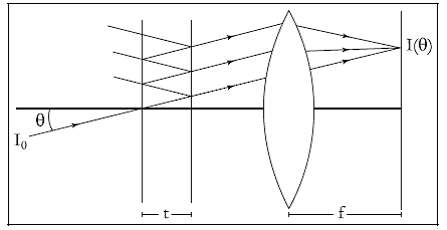
\includegraphics[width = 0.4\textwidth]{FabryPerot.png}
  \begin{center}
  \caption{The Fabry -- P\'{e}rot interferometer. The light enters the interferometer and then exits, interfering with itself and creating Airy Disks.}[\footnotesize{``Atomic Physics.'' - Physics 111-Lab Wiki. UC Berkeley, n.d. Web. 23 Apr. 2015.}]
  \label{FP}
  \end{center}
\end{figure}

A crucial piece of equipment in the Zeeman Effect portion of this experiment is the Fabry -- P\'{e}rot interferometer (Fig~\ref{FP}). This interferometer takes incoming light, reflects it multiple times within its internal mirrors, and then sends the light back out, causing the light to interfere with itself. When one observes the outgoing light from an F--P interferometer, one sees Airy Disks (Fig~\ref{AiryDisk}).

\begin{figure}[h]
  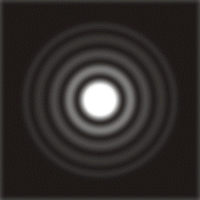
\includegraphics[width = 5 cm]{AiryDisk.png}
  \begin{center}
  \caption{An airy disk, showing interference patterns.}[\footnotesize{``Telescope Equations.": Resolving Power. N.p., n.d. Web. 23 Apr. 2015.}]
  \label{AiryDisk}
  \end{center}
\end{figure}

\subsection{Procedure}

In this experiment, we observed a discharge tube of Helium gas. By passing the light emitted by the Helium gas through a red filter and then through the FP interferometer, we are able to see the Airy Disks. These disks are separated by a quantity that we called $\Delta \sigma$, which has units of cm$^{-1}$. When a magnetic field is applied to the Helium gas, we see the Airy disks split, resembling the Zeeman splitting of the energy levels. In figure~\ref{ZeemanSplitting}, we see that there are two different kind of transitions, $\sigma$ and $\pi$ transitions. $\sigma$ transitions are indicated by the lines that move as the magnetic field is applied to the Helium discharge tube, and are also the transitions that are characterized by $\Delta m_{j} = \pm 1$. On the other hand, the $\pi$ transitions are indicated by the lines that do not move when a magnetic field is applied and the transitions are characterized by $\Delta m_{j} = 0$.
These transitions denote the change in angular momentum. Since $m_j$ is an indicator of the angular momentum of the electron, a transition that yields a change in $m_j$ is a $\sigma$ transition and yields a change in angular momentum. $\pi$ transitions, on the other hand, do not have changes in angular momentum. 

\begin{figure}[tt]
  \begin{center}
    \subfigure[With both $\sigma$ and $\pi$ components. The top and bottom black lines are the $\sigma$ components while the middle line is the $\pi$ component.]{\label{SigmaPi}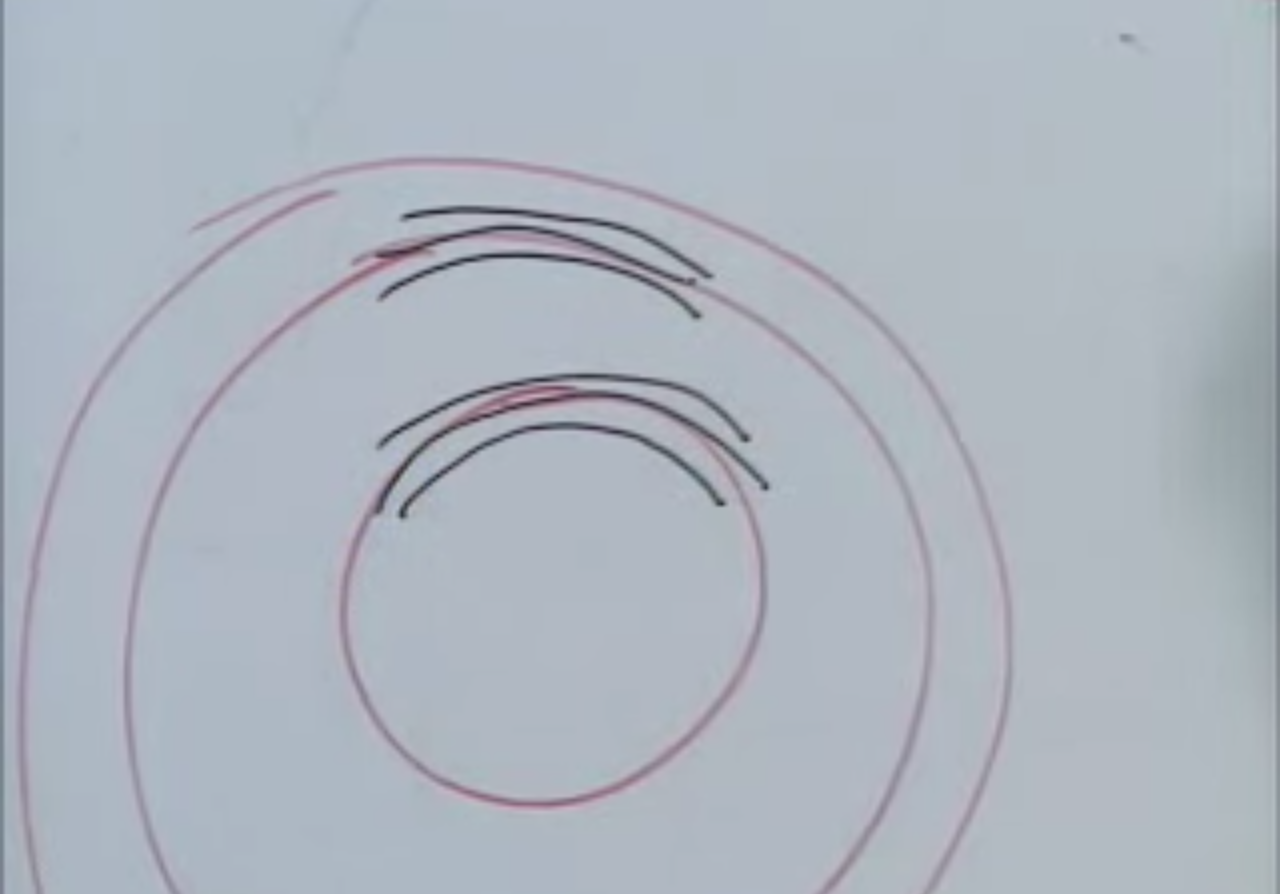
\includegraphics[width=4.1 cm]{sigmapi.png}}
    \subfigure[With the polarizer, eliminating the $\pi$ component.]{\label{Valve}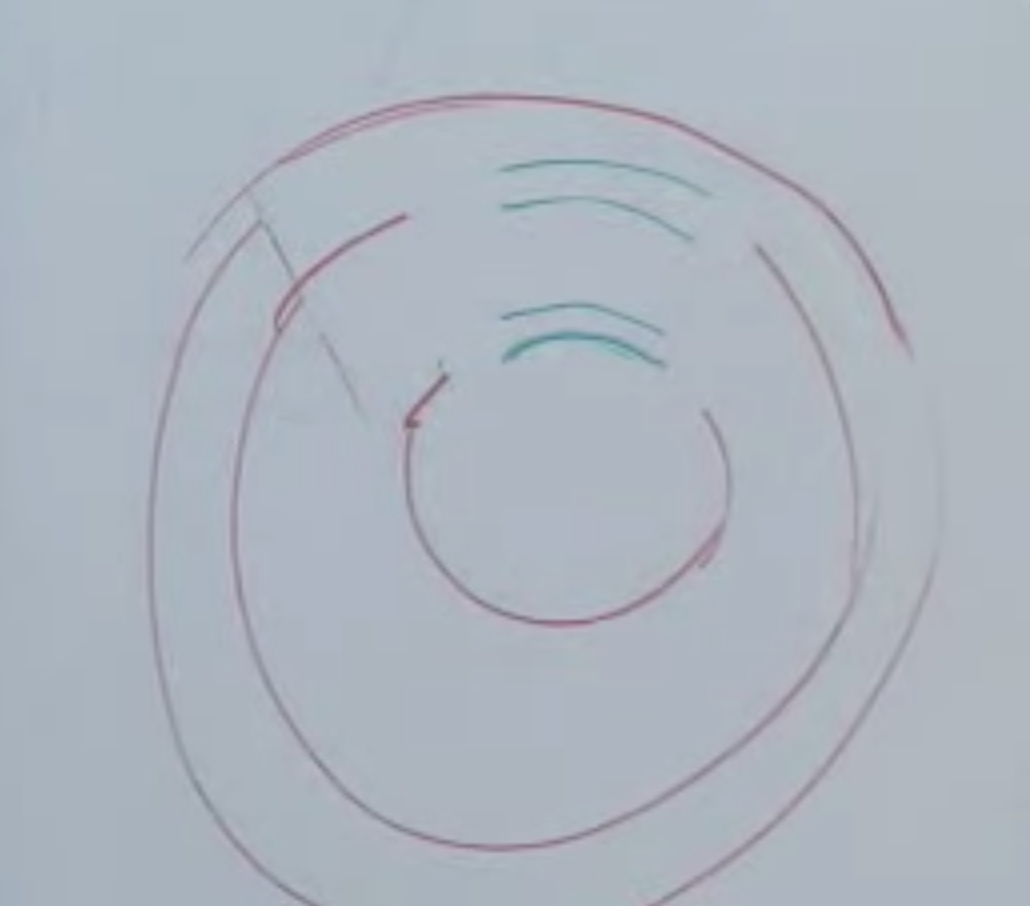
\includegraphics[width=4.1 cm]{justsigma.png}}
  \end{center}
  \caption{Zeeman Splitting showing $\sigma$ and $\pi$ Components}[\footnotesize{``Physics 111: Atomic Physics (ATM) Part 2. Zeeman Effect." YouTube. YouTube, n.d. Web. 23 Apr. 2015.}]
  \label{Sigma and Pi}
\end{figure}

Knowing this about the lines, we can use a circular polarizer to exclude the $\pi$ lines and just observe the $\sigma$ lines. Then we adjusted the magnetic field such that the airy disks were evenly spaced out. This means we had the $\sigma$ lines move $\Delta \sigma / 4$. Afterwards, we included in the $\pi$ lines so that we could find $\Delta \sigma /3$ spacing. Lastly, we found more data for different wavelengths of light. Through all these procedures, we recorded the magnetic field applied whenever we found even spacing. 

\subsection{Analysis}

Using the magnetic field values that we found, we applied them to Equation~\ref{Bohr Magneton}. For $\alpha$, we used the degree of separation of the airy disks; for example, $\alpha$ was $1/3$ if we had the $\pi$ lines or $1/4$ if we did not. All the values for our experiment are found in Table~\ref{ZeemanAnalysis}.

\begin{table}[h]
\begin{tabular}{|l|l|l|l|l|}
\hline
Color  & Order Spacing & B Field (kG) & $\Delta(g m_{j})$ & $\mu_{0}$ (ergs/G) \\ \hline
red    & 0.5 $\pm$ 0.1          & 7.43         & 1.00        & 8.24E-21 $\pm$ 1.65E-21     \\
red    & 0.25 $\pm$ 0.1          & 3.74         & 1.00        & 8.19E-21 $\pm$ 3.28E-21     \\
red    & 0.33 $\pm$ 0.1          & 6.84         & 1.00        & 5.97E-21 $\pm$ 1.79E-21     \\
yellow & 0.25 $\pm$ 0.1          & 11.8         & 0.33        & 7.86E-21 $\pm$ 3.15E-21     \\
yellow & 0.5  $\pm$ 0.1          & 13.8         & 0.33        & 1.35E-20 $\pm$ 2.69E-21     \\ \hline
\end{tabular}
\caption{The magnetic field values indicating certain spacings between Airy Disks. The values in parentheses represent the standard deviations.}
\label{ZeemanAnalysis}
\end{table}

Using these values and taking an average, we determined that the Bohr Magneton is approximately 8.752 $\pm$ 2.512 ergs/G. 

\subsection{Uncertainties}

There were several uncertainties in this experiment. One was the inaccuracy of our eyes being able to tell when airy disks were ``equally spaced''. During our experiment, certain parts of the Airy Disk were evenly spaced while other parts were not (Fig~\ref{BadSpacing}). This made it difficult to determine what we should count as evenly spaced. We concluded that we would use the Airy Disk circles in the outer parts of the image because those disks had higher resolution, which allowed us to make more precise estimates. 

\begin{figure}[ttt]
  \begin{center}
    \subfigure[Half Spacing between Airy Disk circles]{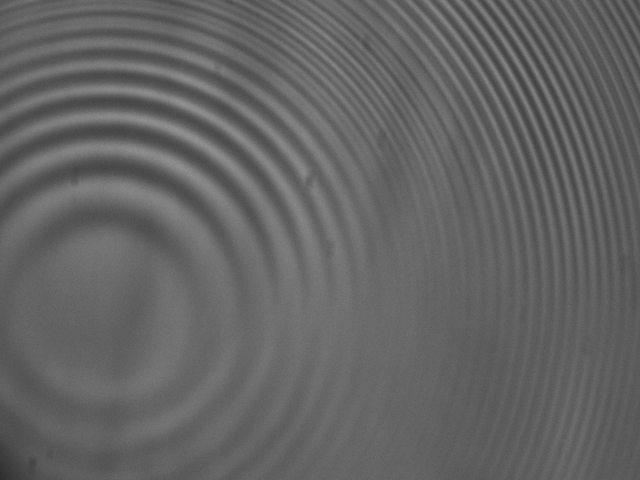
\includegraphics[width=4.1 cm]{Half.png}}
    \subfigure[Quarter Spacing]{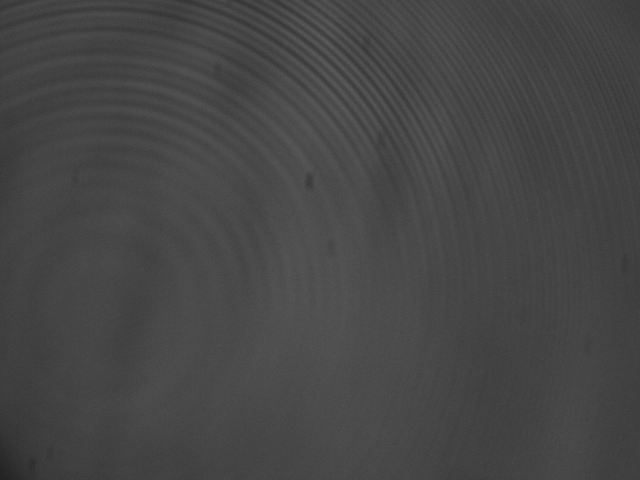
\includegraphics[width=4.1 cm]{Quarter.png}}
    \subfigure[No spacing (Airy disks were moved so much that they overlapped again)]{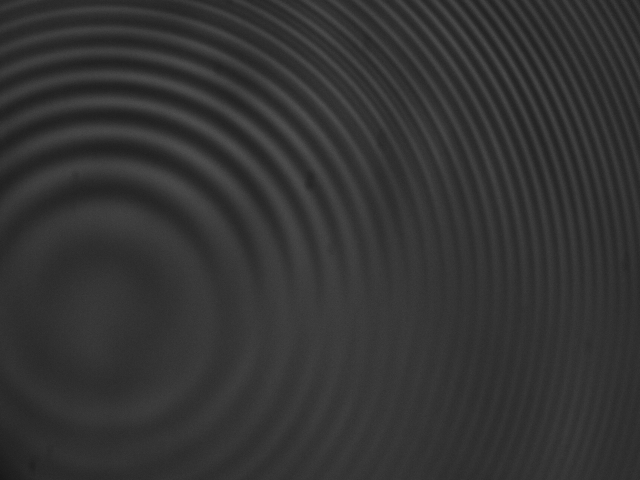
\includegraphics[width=4.1 cm]{No.png}}
  \end{center}
  \caption{Different spaces for different magnetic field strenghts. Notice how ``evenly spaced'' circles in some part of the image are not evenly spaced in other parts.}
  \label{BadSpacing}
\end{figure}

Another area of uncertainty is in the equipment. Equipment error in this part of the lab included a punctured red filter and scratched lenses, both on the camera lenses and focusing lenses. 

With these uncertainties in mind, we included a 0.1 spacing error in our calculations. We chose this value because it was not too large that spacings overlapped with other spacings (for example, 0.5 $\pm$ 0.1 does not overlap with 0.25 $\pm$ 0.1), but is large enough to capture any errors in inconsistent spacing throughout the Airy disks.

\section{Conclusion}

This lab consisted of two parts: one where we studied the Balmer Series of Hydrogen, and one where we studied the Zeeman Effect on a discharge tube of Helium Gas. 

For the first experiment, we used a monochromator and swept through a range of wavelengths using a 300 groove/mm diffraction grating. We first used a discharge tube of Mercury so we could calibrate the monochromator and we found that the wavelength values were, on average, -99.435 nm off. Using this information, we looked at the spectrum for Hydrogen. Since we know that Balmer Series lines finish on the n = 2 state, we used the Rydberg formula, our wavelenght data, and the initial n values to get a linear plot. Through the slope and intercept of that plot, we calculated the Rydberg Constant to be $1.094 \times 10^{7} \pm 2.28 \times 10^{5} $ m$^{-1}$. Uncertainties in that value arise from spectral broadening and scratched lenses. 

For the second experiment, we applied a magnetic field to a discharge tube of Helium. By varying the magnetic field, we could vary how much the Airy Disks moved in and out from each other. By spacing the Airy disks evenly, we were able to determine the Borh Magneton at a certain magnetic field value and with a certain color. This color is important because it indicates the transition between the $g$ and $m_{j}$ values. By calculating the Bohr Magneton for 5 different spacings and colors, we determined that the Bohr Magneton was $8.752 \times 10^{-21} \pm 2.512 \times 10^{-21}$ ergs/G. Uncertainties in that value arise from inconsistent Airy Disk spacing and scratched lenses.

All in all, this experiment is very interesting in that it shows the transitions between different energy levels, including otherwise degenerate levels had it not been for the applied magnetic field. It is a great introduction to optics and atomic physics, and is imperative for the burgeoning physicist that is interested in AMO physics to go through these experiments. However, this research is far from over; in fact, this report warrants further research with better optical equipment that can produce sharper images but also can made the Airy Disks spacing consistent throughout the image. This way we can get more precise and accurate measurements of the Rydberg Constant and Bohr Magneton.

% % %%%%%%%%%%%%%%%%%%%%%%%%%%%%%%%%%%%%%%%%%%%%%%%%%%%%%%%%%%%%%%%%%%%%%%%%%%%%%

\begin{acknowledgments} I acknowledge my lab partner Tanooj Shah for taking data with me and helping me understand the pre-lab questions. I also want to acknowledge GSI Celeste for asking challenging questions but ultimately pushing Tanooj and me to truly understand the lab.
\end{acknowledgments}

\begin{thebibliography}{9}

\bibitem{Website}
  ``Atomic Physics." - \emph{Physics 111-Lab Wiki.} N.p., n.d. Web. 07 May 2015.

\bibitem{1}
  ``Physics 111: Atomic Physics (ATM) Part 1. Balmer Series." \emph{YouTube.} YouTube, n.d. Web. 07 May 2015.

\bibitem{2}
  ``Physics 111: Atomic Physics (ATM) Part 2. Zeeman Effect." \emph{YouTube.} YouTube, n.d. Web. 07 May 2015.

\bibitem{3}
  ``Physics 111: Optical Instruments Lecture." \emph{YouTube.} YouTube, n.d. Web. 07 May 2015.

\bibitem{4}
``Physics 111 Light Sources and Detectors Lecture." \emph{YouTube.} YouTube, n.d. Web. 07 May 2015.

\bibitem{5}
``Physics 111: Energy Levels Lecture Part 1." \emph{YouTube.} YouTube, n.d. Web. 07 May 2015.

\bibitem{6}
``Physics 111: Energy Levels Lecture Part 2." \emph{YouTube.} YouTube, n.d. Web. 07 May 2015.

\bibitem{7}
``Atomic Structure." \emph{Science} 122.3178 (1955): 1010. Web. 7 May 2015.

\end{thebibliography}

\end{document}
